% Packages

% Sets

% Formal statements


\begin{document}
\frame{\titlepage}

\begin{frame}{A goods distribution problem}
	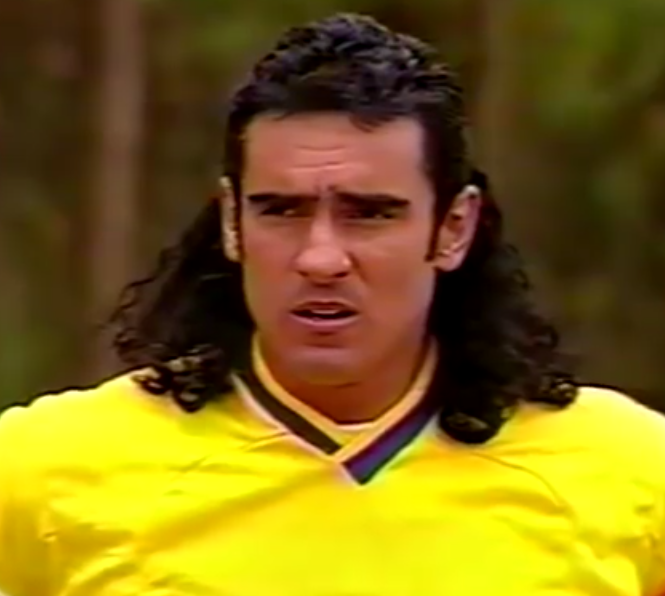
\includegraphics[width= 0.45\textwidth]{pedro_mirandoArco.png}
	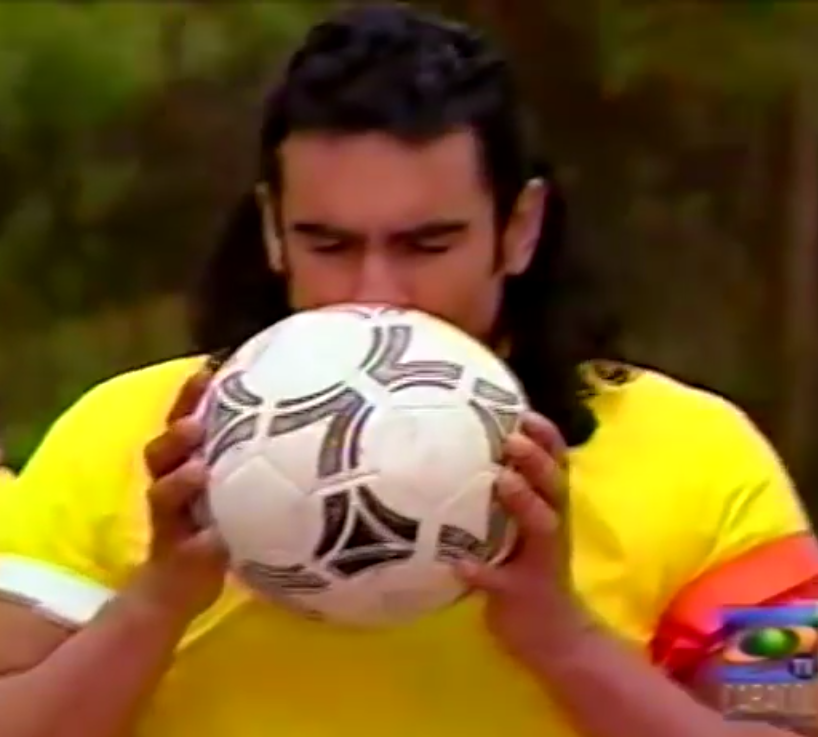
\includegraphics[width= 0.45\textwidth]{pedro_balon.png}
\end{frame}

%

\begin{frame}{A goods distribution problem}
	
\includegraphics[width= 0.25\textwidth]{balonGolty.png}
	\hspace{1cm}
	
\includegraphics[width= 0.25\textwidth]{transporteDeCarga.jpg}

	\bigskip

	\begin{tikzpicture}
		\node[shape= circle, draw, label= above:Ráquira] (Raq) at (0,0) {$\sigma$};
		\node[shape= circle, draw, label= above:Villapinzón, inner sep=2pt] (Vil) at (3,1.5) {$V_1$};
		\node[shape= circle, draw, label= above:Suesca, inner sep=2pt] (Sue) at (6,1.5) {$V_2$};
		\node[shape= circle, draw, label= below:Ubaté, inner sep=2pt] (Uba) at (3,-1.5) {$V_3$};
		\node[shape= circle, draw, label= below:Zipaquirá, inner sep=2pt] (Zip) at (6,-1.5) {$V_4$};
		\node[shape= circle, draw, label= above:Bogotá] (Bog) at (9,0) {$\tau$};
		% Connections
		%% Non-crossing
		\draw [->, >={Stealth[round]}, semithick] (Raq.east) to node [auto] {13} (Vil.west);
		\draw [->, >={Stealth[round]}, semithick] (Vil.east) to node [auto] {14} (Sue.west);
		\draw [->, >={Stealth[round]}, semithick] (Sue.east) to node [auto] {4} (Bog.165);
		\draw [->, >={Stealth[round]}, semithick] (Raq.east) to node [auto] {16} (Uba.west);
		\draw [->, >={Stealth[round]}, semithick] (Uba.east) to node [auto] {12} (Zip.west);
		\draw [->, >={Stealth[round]}, semithick] (Zip.east) to node [auto] {20} (Bog.195);
		%% Crossing
		\draw [->, >={Stealth[round]}, semithick] (Vil.south) to node [auto] {4} (Uba.north);
		\draw [->, >={Stealth[round]}, semithick] (Sue.south) to node [auto] {7} (Zip.north);
		\draw [->, >={Stealth[round]}, semithick] (Sue.210) to node [auto] {9} (Uba.30);
	\end{tikzpicture}
\end{frame}

%

\begin{frame}{The Ford-Fulkerson method}
	\begin{itemize}
		\item Find an augmenting path $p$ from the source $\sigma$ to the sink
			$\tau$.
		\item Augment the flow through each edge of $p$ according to the
			current capacity of the limiting edge.
		\item Repeat until no augmenting paths can be found.
	\end{itemize}
\end{frame}

%

\begin{frame}{The Ford-Fulkerson method}
	\begin{tikzpicture}
		\node[shape= circle, draw, label= above:Ráquira] (Raq) at (0,0) {$\sigma$};
		\node[shape= circle, draw, label= above:Villapinzón, inner sep=2pt] (Vil) at (3,1.5) {$V_1$};
		\node[shape= circle, draw, label= above:Suesca, inner sep=2pt] (Sue) at (6,1.5) {$V_2$};
		\node[shape= circle, draw, label= below:Ubaté, inner sep=2pt] (Uba) at (3,-1.5) {$V_3$};
		\node[shape= circle, draw, label= below:Zipaquirá, inner sep=2pt] (Zip) at (6,-1.5) {$V_4$};
		\node[shape= circle, draw, label= above:Bogotá] (Bog) at (9,0) {$\tau$};
		% Connections
		%% Non-crossing
		\draw [->, >={Stealth[round]}, semithick] (Raq.east) to node [auto] {0/13} (Vil.west);
		\draw [->, >={Stealth[round]}, semithick] (Vil.east) to node [auto] {0/14} (Sue.west);
		\draw [->, >={Stealth[round]}, semithick] (Sue.east) to node [auto] {0/4} (Bog.165);
		\draw [->, >={Stealth[round]}, semithick] (Raq.east) to node [auto] {0/16} (Uba.west);
		\draw [->, >={Stealth[round]}, semithick] (Uba.east) to node [auto] {0/12} (Zip.west);
		\draw [->, >={Stealth[round]}, semithick] (Zip.east) to node [auto] {0/20} (Bog.195);
		%% Crossing
		\draw [->, >={Stealth[round]}, semithick] (Vil.south) to node [auto] {0/4} (Uba.north);
		\draw [->, >={Stealth[round]}, semithick] (Sue.south) to node [auto] {0/7} (Zip.north);
		\draw [->, >={Stealth[round]}, semithick] (Sue.210) to node [auto] {0/9} (Uba.30);
	\end{tikzpicture}
\end{frame}

%

\begin{frame}{The Ford-Fulkerson method}
	\begin{tikzpicture}
		\node[shape= circle, draw, label= above:Ráquira] (Raq) at (0,0) {$\sigma$};
		\node[shape= circle, draw, label= above:Villapinzón, inner sep=2pt] (Vil) at (3,1.5) {$V_1$};
		\node[shape= circle, draw, label= above:Suesca, inner sep=2pt] (Sue) at (6,1.5) {$V_2$};
		\node[shape= circle, draw, label= below:Ubaté, inner sep=2pt] (Uba) at (3,-1.5) {$V_3$};
		\node[shape= circle, draw, label= below:Zipaquirá, inner sep=2pt] (Zip) at (6,-1.5) {$V_4$};
		\node[shape= circle, draw, label= above:Bogotá] (Bog) at (9,0) {$\tau$};
		% Connections
		%% Non-crossing
		\draw [blue, ->, >={Stealth[round]}, thick] (Raq.east) to node [auto] {4/13} (Vil.west);
		\draw [blue, ->, >={Stealth[round]}, thick] (Vil.east) to node [auto] {4/14} (Sue.west);
		\draw [blue, ->, >={Stealth[round]}, thick] (Sue.east) to node [auto] {4/4} (Bog.165);
		\draw [->, >={Stealth[round]}, semithick] (Raq.east) to node [auto] {0/16} (Uba.west);
		\draw [->, >={Stealth[round]}, semithick] (Uba.east) to node [auto] {0/12} (Zip.west);
		\draw [->, >={Stealth[round]}, semithick] (Zip.east) to node [auto] {0/20} (Bog.195);
		%% Crossing
		\draw [->, >={Stealth[round]}, semithick] (Vil.south) to node [auto] {0/4} (Uba.north);
		\draw [->, >={Stealth[round]}, semithick] (Sue.south) to node [auto] {0/7} (Zip.north);
		\draw [->, >={Stealth[round]}, semithick] (Sue.210) to node [auto] {0/9} (Uba.30);
	\end{tikzpicture}
\end{frame}

%

\begin{frame}{The Ford-Fulkerson method}
	\begin{tikzpicture}
		\node[shape= circle, draw, label= above:Ráquira] (Raq) at (0,0) {$\sigma$};
		\node[shape= circle, draw, label= above:Villapinzón, inner sep=2pt] (Vil) at (3,1.5) {$V_1$};
		\node[shape= circle, draw, label= above:Suesca, inner sep=2pt] (Sue) at (6,1.5) {$V_2$};
		\node[shape= circle, draw, label= below:Ubaté, inner sep=2pt] (Uba) at (3,-1.5) {$V_3$};
		\node[shape= circle, draw, label= below:Zipaquirá, inner sep=2pt] (Zip) at (6,-1.5) {$V_4$};
		\node[shape= circle, draw, label= above:Bogotá] (Bog) at (9,0) {$\tau$};
		% Connections
		%% Non-crossing
		\draw [->, >={Stealth[round]}, semithick] (Raq.east) to node [auto] {4/13} (Vil.west);
		\draw [->, >={Stealth[round]}, semithick] (Vil.east) to node [auto] {4/14} (Sue.west);
		\draw [->, >={Stealth[round]}, semithick] (Sue.east) to node [auto] {4/4} (Bog.165);
		\draw [blue, ->, >={Stealth[round]}, thick] (Raq.east) to node [auto] {12/16} (Uba.west);
		\draw [blue, ->, >={Stealth[round]}, thick] (Uba.east) to node [auto] {12/12} (Zip.west);
		\draw [blue, ->, >={Stealth[round]}, thick] (Zip.east) to node [auto] {12/20} (Bog.195);
		%% Crossing
		\draw [->, >={Stealth[round]}, semithick] (Vil.south) to node [auto] {0/4} (Uba.north);
		\draw [->, >={Stealth[round]}, semithick] (Sue.south) to node [auto] {0/7} (Zip.north);
		\draw [->, >={Stealth[round]}, semithick] (Sue.210) to node [auto] {0/9} (Uba.30);
	\end{tikzpicture}
\end{frame}

%

\begin{frame}{The Ford-Fulkerson method}
	\begin{tikzpicture}
		\node[shape= circle, draw, label= above:Ráquira] (Raq) at (0,0) {$\sigma$};
		\node[shape= circle, draw, label= above:Villapinzón, inner sep=2pt] (Vil) at (3,1.5) {$V_1$};
		\node[shape= circle, draw, label= above:Suesca, inner sep=2pt] (Sue) at (6,1.5) {$V_2$};
		\node[shape= circle, draw, label= below:Ubaté, inner sep=2pt] (Uba) at (3,-1.5) {$V_3$};
		\node[shape= circle, draw, label= below:Zipaquirá, inner sep=2pt] (Zip) at (6,-1.5) {$V_4$};
		\node[shape= circle, draw, label= above:Bogotá] (Bog) at (9,0) {$\tau$};
		% Connections
		%% Non-crossing
		\draw [blue, ->, >={Stealth[round]}, thick] (Raq.east) to node [auto] {11/13} (Vil.west);
		\draw [blue, ->, >={Stealth[round]}, thick] (Vil.east) to node [auto] {11/14} (Sue.west);
		\draw [->, >={Stealth[round]}, semithick] (Sue.east) to node [auto] {4/4} (Bog.165);
		\draw [->, >={Stealth[round]}, semithick] (Raq.east) to node [auto] {12/16} (Uba.west);
		\draw [->, >={Stealth[round]}, semithick] (Uba.east) to node [auto] {12/12} (Zip.west);
		\draw [blue, ->, >={Stealth[round]}, thick] (Zip.east) to node [auto] {19/20} (Bog.195);
		%% Crossing
		\draw [->, >={Stealth[round]}, semithick] (Vil.south) to node [auto] {0/4} (Uba.north);
		\draw [blue, ->, >={Stealth[round]}, thick] (Sue.south) to node [auto] {7/7} (Zip.north);
		\draw [->, >={Stealth[round]}, semithick] (Sue.210) to node [auto] {0/9} (Uba.30);
	\end{tikzpicture}
\end{frame}

%

\begin{frame}{Ford-Fulkerson: Formal questions}
	\begin{itemize}
		\item How should we define ``flow''?
		\item What do we mean by ``augmenting path''?
		\item What do we mean by ``limiting edge''?
		\item How can we be sure that the algorithm stops?
		\item How can we be sure that Ford-Fulkerson provides an optimal solution?
		\item According to what criteria can we claim that Ford-Fulkerson is ``efficient''?
	\end{itemize}
\end{frame}

%

\begin{frame}{Flow networks}
	A \emph{flow network} is the same as a directed graph with weights. Namely,
	it is the data $(N, A, \mathbf{w})$ where
	\begin{itemize}
		\item $N$ is a finite set whose elements are called \emph{nodes}
		\item $A \subset N \times N - \triangle_N$ is the set of \emph{edges}
		\item $\mathbf{w}: A \to \Zpos$ is the function of \emph{weights}.
	\end{itemize}
\end{frame}

%

\begin{frame}{Computational complexity}
	
\includegraphics[width= 0.6\textwidth]{mario.png}

	\bigskip

	\pause
	We've used notation such as $O$ and $\Omega$ to describe the worst-case complexity of
	\emph{algorithms}. We must now turn to the complexity of \emph{computational problems}. 
\end{frame}

%

\begin{frame}{Computational complexity --- \emph{Church-Turing thesis and models of computation}}
	\textbf{Models of computation}
	\begin{itemize}
		\item Turing machines \checkmark (ISIS1106)
		\item RAM instructions \checkmark (Every other course)
		\item Lambda calculus
		\item Arithmetic circuits
		\item Boolean circuits
	\end{itemize}

	\bigskip

	\pause
	The \textbf{Church-Turing thesis} says that any two of these models are equivalent.

	\bigskip

	\pause
	Our discussion of computational complexity and so-called ``intractability'' will be in
	terms of the \emph{RAM} model of computation. 
\end{frame}

%

\begin{frame}{RAM instructions model of computation}
	\begin{itemize}
		\item We will use a \textbf{fixed programming language \underline{with types}},
			very Java-like.
		\item[] {\scriptsize \it *We may nonetheless occasionally discuss some statements
			in terms of Turing machines*}
	\end{itemize}
\end{frame}

%

\begin{frame}{Decision problems}
	\begin{defn}
		Let $\hat{X}$ be a type of our programming language and let $X \subset \hat{X}$. The
		\emph{decision problem} defined by $X$ consists of assigning \textbf{true} or 
		\textbf{false} to the expression $x \in X$ for all $x \in \hat{X}$. 
	\end{defn}

	\begin{exl}
		\begin{enumerate}
			\item $\hat{X}= \ZZ$, $X=$ Primes.
			\item $\hat{X}= \mathtt{Graph}$, $X= \mathtt{connGraph}$. Namely, the
				problem of deciding whether or not a graph is connected.
			\item $\hat{X}= \mathtt{String}$, $X=$ Python programs that stop.
		\end{enumerate}
	\end{exl}
\end{frame}

%

\begin{frame}{Decision problems - computability}
	\begin{defn}
		The decision problem $X \subset \hat{X}$ is \emph{computable} if there exists
		a program
		\[
			\mathbf{boolean}\ \mathtt{checkX}(\hat{X}\ x)
		\]
	\end{defn}
\end{frame}
\end{document}
